\documentclass [letterpaper] {article}
\usepackage{indentfirst}
\usepackage{amsmath}%Math
\usepackage{amsfonts}
\usepackage{amssymb}
\usepackage{geometry}%Margins
%\geometry{left=2.54cm,right=2.54cm,top=2.54cm,bottom=2.54cm}
\usepackage{setspace}%LineSpacing
\renewcommand{\baselinestretch}{1}
\usepackage{booktabs}%Table
\usepackage{array}%TableHeight
\renewcommand\arraystretch{1}
\usepackage{graphicx}%Figure
\usepackage{subfig}
\usepackage{listings}
\lstset{
	basicstyle = \ttfamily
}
\bibliographystyle{unsrt}

\begin {document}

\setcounter{page}{1}
\pagestyle{plain}%LocationOfPageNumber

\begin{center}
\textbf{\huge{STAT GR5221 Project}}
\linebreak

\large{Runfeng Tian (rt2755)}
\end{center}

\section{Introduction}
\subsection{Data description}

Here we have a dataset containinng Nasdaq-100 index from 2008-01-02 to 2020-05-01. Nasdaq-100 index is a stock market index made up of 103 equity securities issued by 100 of the largest non-financial American and international companies such as Amazon, Apple inc. and Baidu. It is an important indication of the trend of American stock market. 

\subsection{Objective}

\indent In this project, whether time series model ARMA and GARCH can perform consistently when volatility changes abruptly in a very short time will be checked.\\
\begin{figure}[htp]
\centering
\subfloat[Nasdaq-100 index trend]{
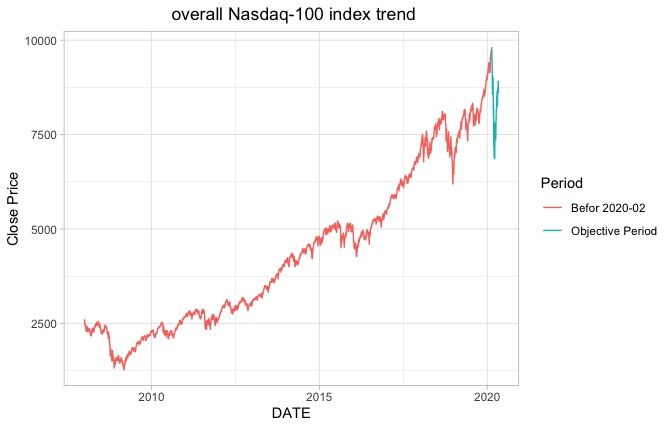
\includegraphics[width = 7cm,height=5cm]{Plots/Pricetrend.jpeg}
}
\quad
\subfloat[Log return trend of Nasdaq-100 trend]{
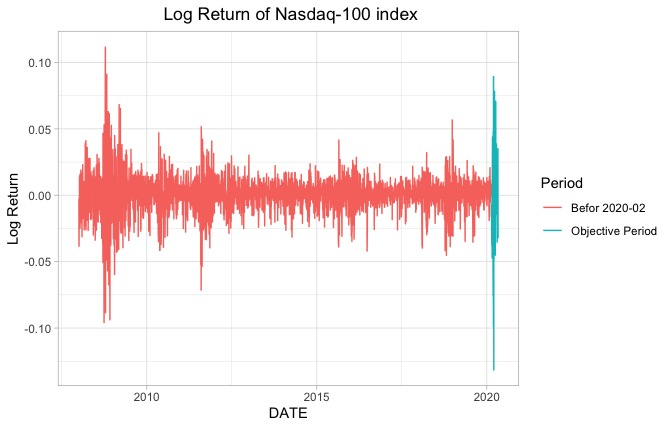
\includegraphics[width = 7cm,height=5cm]{Plots/LogReturn.jpeg}
}
\caption{Overall trend plot}
\end{figure}

Beginning in 2020-02, the pandemic of COVID-19 continued to impact the american stock market. From Figure1, we can find that the blue part in plot (a) and plot(b) have a high volatitlity different from former period. Such uncertainty in stock market is both a challenge and opportunity for investment. In this project, I will utilize time series models ARMA and GARCH trained on former data, and then test the model performances through forecasting on the latest data observations (check the accurracy of forecast in such a period with high volatility).




\section{Exploratory data analysis and modeling}
\subsection{Data clean and transofrmation}
This dataset containing total 3105 observations of Nasdaq-100 index from 2008-01-02 to 2020-05-01. After checking, I find that there are 3 missing values at time nodes:2016-12-14, 2017-09-06 amd 2020-04-02.\\
\indent To deal with missing values, one can implement several methods such as deleting the observations, forward filling, backward filling and etc. Here, since the missing values are not neighbour to each other, it is easy to substitute the missing values with mean of the former and next non-missing values cloest to that data points.\\
\indent In other words, let the $P_t$ denote the original Nasdaq-100 index. Missing data points $P_{t_i}$ can be represented as:
\[
P_{t_i}=\frac {P_{t_i+1}+P_{t_i-1}}{2}
\]

\begin{figure}[htp]
	\centering
	\subfloat[Orginal $P_t$ trend]{
		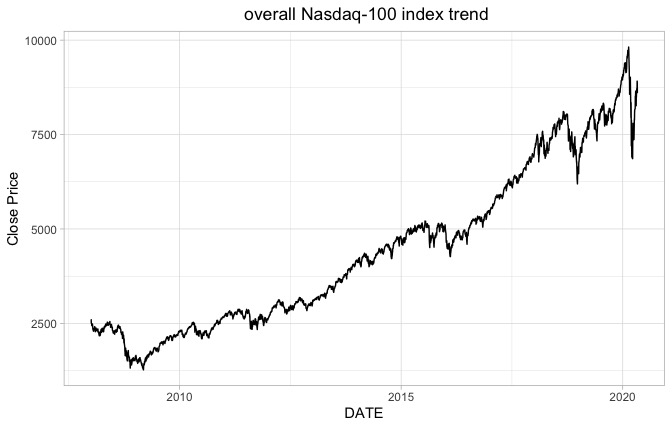
\includegraphics[width = 7cm,height=5cm]{Plots/Original_Pt.jpeg}
	}
	\quad
	\subfloat[$R_t$ trend]{
		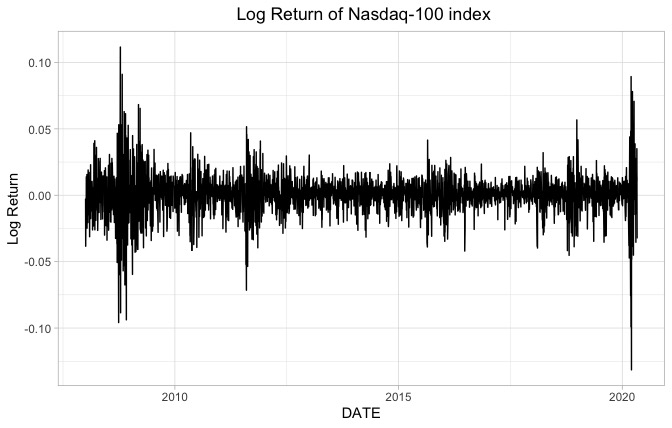
\includegraphics[width = 7cm,height=5cm]{Plots/Rt.jpeg}
	}
	\caption{Data Transformation Plot}
\end{figure}

In Figure 2 part(a), there is an obvious increase trend, which means that the original Nasdaq-100 index data is non-stationary. In order to apply time series model such as ARMA or Garch on the series. Data transformation is necessary.\\
Let $r_t$ denote the log return of the original price data $P_t$
\[
r_{t}=\frac {P_{t}}{P_{t-1}}\quad t=2,3,..,3105
\]

\indent Here, due to several beneficiary properites of log return, such as stationarity, gaussain property(if log$Pt$ is gaussain, then $r_{t}=\frac {P_{t}}{P_{t-1}} $is also gaussain. Hence, the compound log return from $t1$ to $t2$ is $log\frac{P_{t2}}{P_{t1}}=r_{t2}+r_{t2-1}+...+r_{t1+1}$) , it is convenient and meaningful to do time series analysis on squence {$r_t$} instead of {$P_t$}.\\
\indent In Figue2(b),  there is no obvious increase and decrease trend in ${r_t}$. So we can generally consider the sequence is stationary, but the volatilties vareis from periods to periods. Theoritically, GARCH model will have higher performance in such data than ARMA do. 

\subsection{Modeling and Forecast Evaluation}
\subsubsection{Modeling on the whole data set}
In this section, the whole dataset with 3105 observations is split into training data before 2020-02-20 and test data from 2020-02-20 to 2020-05-01. Then ARMA and ARMA-GARCH models are trained seperately on training set.\\
First, train Model 1 ARAMA(4,5). The model odrder is selected based on AIC.

\begin{equation}
\begin{aligned}
\mathrm{\bold{Model\ 1}\ ARMA(4,5)}:\; \phi(B)r_t = \phi_0+\theta (B)w_t, \quad w_t \sim N(0, \sigma_{w}^2)\\
where\quad  \phi(z)=1-\phi_1z-\phi_2z^2-\phi_3z^3-\phi_4z^4,\\ \theta(z)=1+\theta_1z+\theta_2z^2+\theta_3z^3+\theta_4z^4+\theta_5z^5\\
\phi_0\ is\ intercept
\end{aligned}
\end{equation}

The estimations of Model 1 are following:
\begin{lstlisting}
Coefficients:
         ar1      ar2      ar3      ar4     ma1     ma2     ma3     ma4
      -0.7325  -0.6665  -0.9797  -0.2389  0.6592  0.5667  0.9200  0.1372
s.e.   0.3170   0.1762   0.1857   0.2911  0.3166  0.1572  0.1767  0.2850
         ma5     intercept
      -0.0873      4e-04
s.e.   0.0272      2e-04

sigma^2 estimated as 0.0001757:  log likelihood = 8867.43,  aic = -17712.85
\end{lstlisting}	

Second, implement ARMA(4,5)-GARCH(1,1) on training data.
\begin{equation}
\begin{aligned}
\mathrm{\bold{Model\ 2}\ ARMA(4,5)-GARCH(1,1)}:\; \phi(B)r_t = \phi_0+\theta (B)w_t, \quad w_t \sim N(0, \sigma_{w}^2)\\
where\quad  \phi(z)=1-\phi_1z-\phi_2z^2-\phi_3z^3-\phi_4z^4,\\ \theta(z)=1+\theta_1z+\theta_2z^2+\theta_3z^3+\theta_4z^4+\theta_5z^5\\
\phi_0\ is\ intercept\\\\
w_t=sigma_t\epsilon_t, \ \epsilon_t \sim N(0,1)\\
\sigma_{t}^2=\alpha_0+\alpha_1w_{t-1}^2+\beta_1\sigma_{t-1}^2
\end{aligned}
\end{equation}

The estimations of Model 2 are following:
\begin{lstlisting}
Coefficients:
       ar1      ar2      ar3      ar4     ma1     ma2     ma3     ma4
     -0.1038 -0.2323   0.7867   0.4298  0.0582  0.2099 -0.8096 -0.4091 
s.e.  0.0001  0.0239   0.0132   0.0122  0.0261  0.0200  0.0227  0.0001
       ma5    intercept omega   alpha1    beta1
      0.0127  0.0009   0.0000   0.1229  0.8521
s.e.  0.0195   0.0001  0.0000   0.0116  0.0146


\end{lstlisting}	
	

\subsection{Model diagnostic and forecast on test set}
\subsubsection{Model diagnostic}
After modeling on trainig set, a series  of goodness of fit check processes such as Ling-jun box test are carried. 

\begin{figure}[htp]
	\centering
	\subfloat[ARMA(4,5) Residual Check]{
		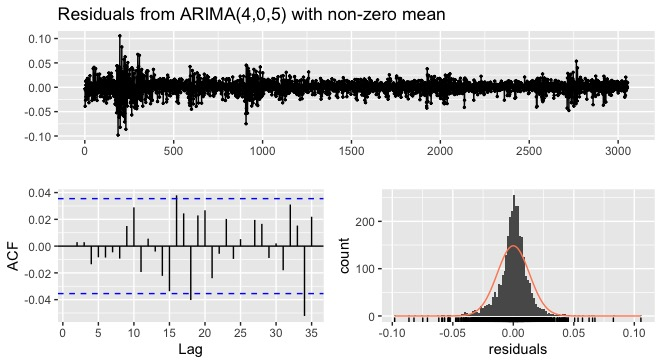
\includegraphics[width = 7cm,height=5cm]{Plots/ARMA(4,5).jpeg}
	}
	\quad
	\subfloat[ARMA(4,5)-GARCH(1,1) Residual Check]{
		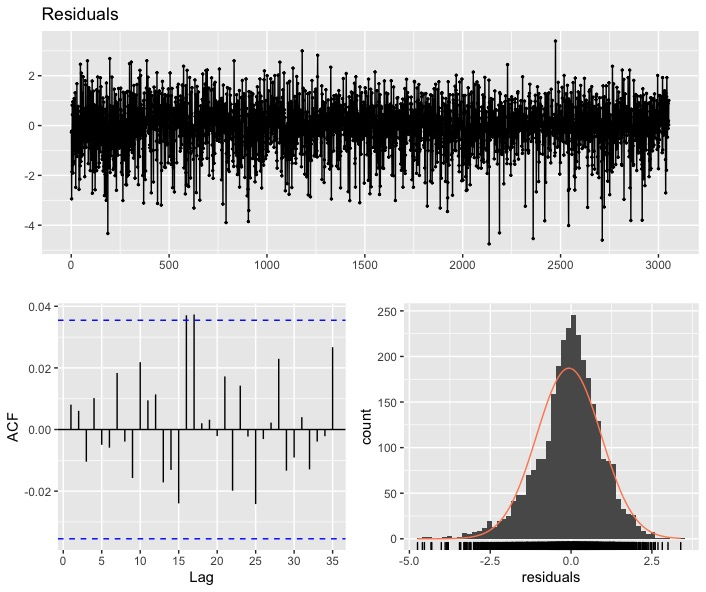
\includegraphics[width = 7cm,height=5cm]{Plots/ARMA-GARCH.jpeg}
	}
	\caption{Goodness of Fit Check Plot}
\end{figure}

From Figure3 residual plots and ACF plots, the reisudals of both ARMA(4,5) and ARMA(4,5)-GARCH(1,1)  are generally uncorrelated.  In addition, the both Ling-jung Box tests fail to reject null hypothesis: the residuals are uncorrelated under the significance level 0.05. Therefore, the 2 models are considered well-fitted.

\begin{lstlisting}
Lingjun-Box test:
ARMA(4,5): Q*= 5.9434, p-value=0.1144
ARMA(4,5)-GARCH(1,1): Q*=0.19952, p-value=0.6551
\end{lstlisting}	


\subsubsection{Model forecast on test set}
After applying goodness of fit check to model 1 and model 2, in this part, the model performances on test set are evaluated which are the key point of this project. The test data containing 51 observations from 2020-02-20 to 2020-05-01 which is the period with much higher volatility than former period. 51-step forecast are conducted on both model 1 and model 2. \\
After forecaste, both forecaste and real log return values are tranformed into commoly used return. Let $\hat {r_t}$ and $r_t$ respectively denote forecast value and real value of log return. Then return value $R_t$ is expressed as:\\
$\hat {R_t}=e^{\hat{r_t}}-1$,  $R_t=e^{r_t}-1$\\
\indent In Figure 4, both forecasting values in 2 models(red line) are nearly 0 for each data point. The shadow dondary in the plots represent 95 percent confident interval for the real return value. But few of real value(blue points) fall into the confident interval. Such results mean that both ARMA(4,5) and ARMA(4,5)-GARCH(1,1) trained on whole dataset perform poorly on forecast. 

\begin{figure}[htp]
	\centering
	\subfloat[ARMA(4,5) 51-step forecast]{
		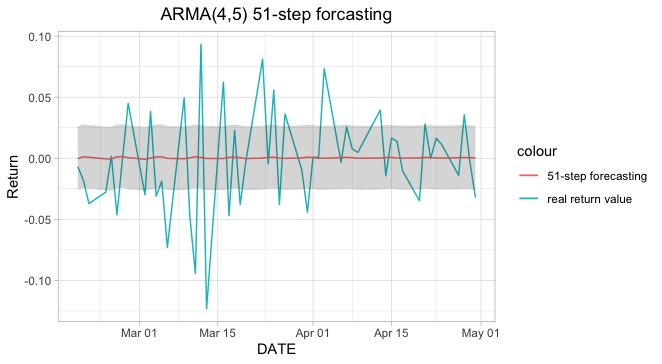
\includegraphics[width = 7cm,height=5cm]{Plots/ARMA(4,5)forecast.jpeg}
	}
	\quad
	\subfloat[ARMA(4,5)-GARCH(1,1) 51-step forecast]{
		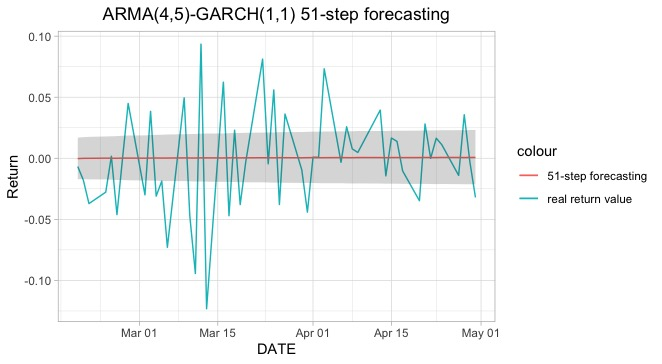
\includegraphics[width = 7cm,height=5cm]{Plots/ARMA-GARCH_forecast_whole.jpeg}
	}
	\caption{Forecast on test data}
\end{figure}

The poor forecast can be caused by several possible factors: first, the models we choose are  inapproriate for the struture of the data. Second, the way of model fitting is in approriate. It is likely that the model trained on long history data can hardly size the abrupt change in vary short time. In this case, the models fail to explain the sudden volatility change leading to poor forecast. 

\subsection{Modeling  on data from 2019-01-02 to 2020-05-01 and forecaste}
In this section, modeling training the whole dataset, the same models in 2.2.1 are modeled on a subset of whole dataset containing relatively latest observations. The data containing 336 observations from 2019-01-02 to 2020-05-01 are split into training set including first 316 points and test set including last 20 points.\\
\subsubsection{Modeling on smaller dataset}
$\bold{Model 3}$: ARMA(4,5) trained on  subset of data:

\begin{lstlisting}
Coefficients:
         ar1      ar2      ar3      ar4     ma1     ma2     ma3     ma4     
      -2.2287  -2.1512  -1.0017  -0.2166  2.0249  1.8683  1.0344  0.6069  
s.e.   0.2055   0.4912   0.4685   0.1783  0.2019  0.4420  0.3808  0.1495  
         ma5  intercept
       0.3515    3e-04
       0.0780    9e-04
sigma^2 estimated as 0.0002228:  log likelihood = 878.83,  aic = -1735.67
\end{lstlisting}	


$\bold{Model 4}$: ARMA(4,3)-GARCH(1,1) (here the model order of q order of ARMA(4,5)-GARCH(1,1) has been lowered because for dataset with smaller number of observations, ARMA-GARCH is reasonable to be simpler):
\begin{lstlisting}
Coefficients:
         ar1      ar2      ar3      ar4     ma1     ma2     ma3     
      -1.7431   -1.2770  -0.4744  -0.1984 1.7002  1.1337  0.1999
s.e.   0.0402    0.1767   0.2020   0.0711 0.1373  0.1612  0.0597
      intercept  omega    alpha1    beta1
       0.0022    0.0000   0.4273   0.5717
s.e.   0.0003    0.0000   0.0846   0.0487
\end{lstlisting}
	

\subsubsection{Model 3 and 4 evaluation based on forecast}
In order to check wether smaller data set inluding  latest observations can improve forecast when volatility changes abruply, similar forecast are carried on test data set(20 observations, 2020-04-03 to 2020-05-01).

\begin{figure}[htp]
	\centering
	\subfloat[ARMA(4,5) 20-step forecast]{
		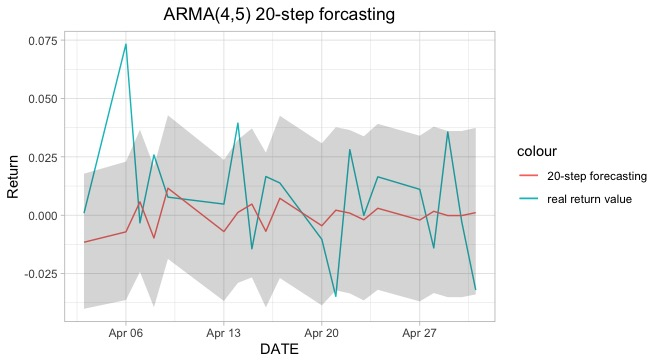
\includegraphics[width = 7cm,height=5cm]{Plots/ARMA(4,5)forecast_small.jpeg}
	}
	\quad
	\subfloat[ARMA(4,5)-GARCH(1,1) 20-step forecast]{
		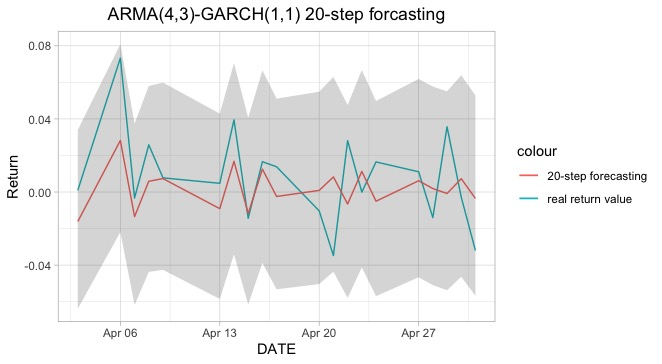
\includegraphics[width = 7cm,height=5cm]{Plots/ARMA(4,3)-GARCH(1,1)_forecast_small.jpeg}
	}
	\caption{Model 3 and Model 4 Forecast on test data from 2020-04-03 to 2020-05-01}
\end{figure}
From Figure5, we can find that most real values of return fall into the 95\% confidence interval, which means forecast performances of model 3 and model 4  are generally better than model 1 and 2 trained on whole history data. In addition, model 4 performs better on the test data than ARMA(4,5) does because in Figure5(b), the changing pattern of forecast values are similar to that of real values. 

\begin{figure}[htp]
	\centering
	\subfloat[ARMA(4,5) 20-step forecast residuals]{
		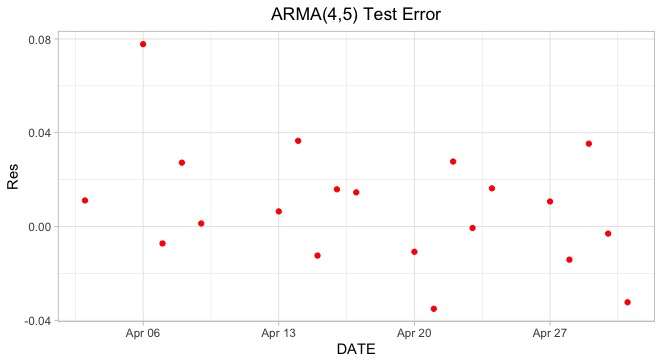
\includegraphics[width = 7cm,height=5cm]{Plots/ARMAres_plot.jpeg}
	}
	\quad
	\subfloat[ARMA(4,5)-GARCH(1,1) 20-step forecast residuals]{
		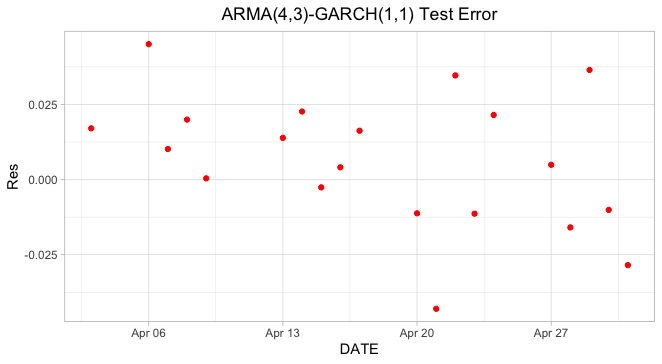
\includegraphics[width = 7cm,height=5cm]{Plots/ARMA(4,3)-GARCH(1,1)TestError.jpeg}
	}
	\caption{Model 3 and Model 4 test error}
\end{figure}

 The residuals plot of model 3 and model 4 forecasts also show that ARMA(4,3)-GARCH(1,1) model forecast more accurately on the test set than ARMA(4,5) does, since the range of most residuals in Figure6(b) ([-0.025,0.025]) is smaller than that in Figure6(a)([-0.04,0.04]).
 
 
 
 \section{Conclusion}
 Based on the analysis and model comparisons in the former sections, it is concluded that time series models: ARMA and GARCH trained on relatively small dataset can perform better in forecasting than those trained on a dataset with certainly long duration in terms of forecast on a period during which the volatility changes abruptly . That is because  for data with volitility varies from period to period, the former observations in the sequence may contain too much useless information  would lead to incorrect model fitting. On the other hand, latest data is more useful in correctly desribing current and future market situation.\\
 \indent Furthermore, compared to ARMA model, ARMA-GARCH model taking volatility changes into account is likely to achieve a better forecast on data with high volatility. In general, for short term forecast, GARCH model can be a very powerful model.
 
 \section{Extension and future research direction}
In former discussion and analysis, wether ARMA and ARMA-GARCH model can perform well under the circumstances when volatilities vary in different periods is explored and one can utilize a smaller dataset containing latest data to improve forecast accuracy . Some researchers have provided other methods such as 
adding dummy variables respresenting the features of different volatilities to GARCH model. They argued that the volatility persistence has been overestimated by GARCH model and taking breakpoints for volatility differences into consideration can effectively correct the volatility persistence in GARCH(\cite{num1}). Therefore, we can introduce the new model into modeling comparisons and evaluate models in term of forecast. In addition, stock arbitrage method can be designed based on the forecasting return if its accuracy  is high enough.


\bibliography{ref}




\end {document}